\section{Constrained Optimization:Lagrange Multipliers} \label{S:10.8.Lagrange_Multipliers}

\vspace*{-14 pt}
\framebox{\hspace*{3 pt}
\parbox{6.25 in}{\begin{goals}
  \item What geometric condition enables us to optimize a function $f=f(x,y)$ subject to a constraint given by $g(x,y) = k$, where $k$ is a constant?
  \item How can we exploit this geometric condition to find the extreme values of a function subject to a constraint?
\end{goals}} \hspace*{3 pt}}

\subsection*{Introduction}

We previously considered how to find the extreme values of functions on both unrestricted domains and on closed, bounded domains. Other types of optimization problems involve maximizing or minimizing a quantity subject to an external constraint. In these cases the extreme values frequently won't occur at the points where the gradient is zero, but rather at other points that satisfy an important geometric condition. These problems are often called \emph{constrained optimization} problems and can be solved with the method of Lagrange Multipliers, which we study in this section. 

\begin{pa} \label{PA:10.8}  According to U.S.~postal regulations, the girth plus the length of a parcel sent by mail may not exceed 108 inches, where by ``girth'' we mean the perimeter of the smallest end.  Our goal is to find the largest possible volume of a rectangular parcel with a square end that can be sent by mail.\footnote{We solved this applied optimization problem in single variable \emph{Active Calculus}, so it may look familiar. We take a different approach in this section, and this approach allows us to view most applied optimization problems from single variable calculus as constrained optimization problems, as well as provide us tools to solve a greater variety of optimization problems.} If we let $x$ be the length of the side of one square end of the package and $y$ the length of the package, then we want to maximize the volume $f(x,y) = x^2y$ of the box subject to the constraint that the girth ($4x$) plus the length ($y$) is as large as possible, or $4x+y = 108$.  The equation $4x + y = 108$ is thus an external constraint on the variables. 
    \ba
    \item The constraint equation involves the function $g$ that is given by
    \[g(x,y) = 4x+y.\]
    Explain why the constraint is a contour of $g$, and is therefore a two-dimensional curve.

  \begin{figure}[ht]
  \begin{center}
    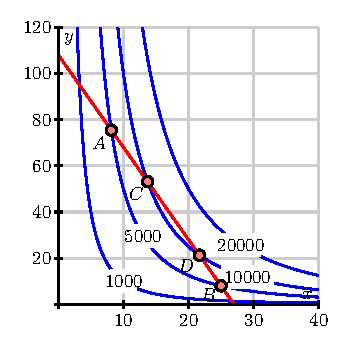
\includegraphics{figures/fig_10_8_postal.eps}
  \end{center}
  \caption{Contours of $f$ and the constraint equation $g(x,y) = 108$.}
  \label{F:10.8.preview}
  \end{figure}

    \item Figure \ref{F:10.8.preview} shows the graph of the constraint equation $g(x,y) = 108$ along with a few contours of the volume function $f$.  Since our goal is to find the maximum value of $f$ subject to the constraint $g(x,y) = 108$, we want to find the point on our constraint curve that intersects the contours of $f$ at which $f$ has its largest value. 
	\begin{enumerate}[i.]
	\item Points $A$ and $B$ in Figure \ref{F:10.8.preview} lie on a contour of $f$ and on the constraint equation $g(x,y) = 108$. Explain why neither $A$ nor $B$ provides a maximum value of $f$ that satisfies the constraint. 
	\item Points $C$ and $D$ in Figure \ref{F:10.8.preview} lie on a contour of $f$ and on the constraint equation $g(x,y) = 108$. Explain why neither $C$ nor $D$ provides a maximum value of $f$ that satisfies the constraint. 
	\item Based on your responses to parts i. and ii., draw the contour of $f$ on which you believe $f$ will achieve a maximum value subject to the constraint $g(x,y) = 108$. Explain why you drew the contour you did. 
	\end{enumerate}
	

\item Recall that $g(x,y) = 108$ is a contour of the function $g$, and that the gradient of a function is always orthogonal to its contours. With this in mind, how should $\nabla f$ and $\nabla g$ be related at the optimal point? Explain. 


    \ea
\end{pa} 

\begin{activitySolution} 
    \ba
    \item A contour is a curve obtained by setting the dependent variable equal to a constant. So if $g(x,y) = 4x+y$, then the equation $108 = 4x+y = g(x,y)$ is a contour of $g$.


    \item Notice that there are contours of $f$ that intersect the constraint with higher values of $f$ than occur at points $A$, $B$, $C$, or $D$. It appears that that maximum value of $f$ that we want will occur at a point where the contour of $f$ intersects the constraint at only one point -- or when the contour of $f$ is tangent to the constraint.


\item When the graph of the constraint is tangent to a level curve of $f$, then the two curves will have the same direction at this point. This implies any two vectors that are orthogonal to these level curves will have to be parallel at the point of tangency. So $\nabla f$ and $\nabla g$ will have to be parallel at the point of tangency.


    \ea
\end{activitySolution}
\afterpa 

\subsection*{Constrained Optimization and Lagrange Multipliers}

In Preview Activity \ref{PA:10.8}, we considered an optimization problem where there is an external constraint on the variables, namely that the girth plus the length of the package cannot exceed 108 inches. We saw that we can create a function $g$ from the constraint, specifically $g(x,y) = 4x+y$.  The constraint equation is then just a contour of $g$, $g(x, y) = c$,  where $c$ is a constant (in our case 108). Figure \ref{F:10.8.Lagrange1} illustrates that the volume function $f$ is maximized, subject to the constraint $g(x, y) = c$, when the graph of $g(x, y) = c$ is tangent to a contour of $f$. Moreover, the value of $f$ on this contour is the sought maximum value.
\begin{figure}[h]
\begin{center}
%\resizebox{!}{2.0in}{\includegraphics{10_8_Lagrange1}}
  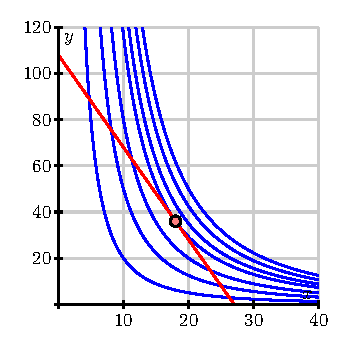
\includegraphics{figures/fig_10_8_postal_solution.eps}
\end{center}
\caption{Contours of $f$ and the constraint contour.}
\label{F:10.8.Lagrange1}
\end{figure}
To find this point where the graph of the constraint is tangent to a contour of $f$, recall that $\nabla f$ is perpendicular to the contours of $f$ and $\nabla g$ is perpendicular to the contour of $g$. At such a point, the vectors $\nabla g$ and $\nabla f$ are parallel, and thus we need to determine the points where this occurs. Recall that two vectors are parallel if one is a nonzero scalar multiple of the other, so we therefore look for values of a parameter $\lambda$ that make
\begin{equation}
\nabla f = \lambda \nabla g.\label{eq:10.8.Lagrange_ex1}
\end{equation}
The constant $\lambda$ is called a \emph{Lagrange multiplier}\index{Lagrange multiplier}.

To find the values of $\lambda$ that satisfy (\ref{eq:10.8.Lagrange_ex1}) for the volume function in Preview Activity~\ref{PA:10.8}, we calculate both $\nabla f$ and $\nabla g$. Observe that
\[\nabla f = 2xy \vi + x^2 \vj \ \ \ \ \text{ and } \ \ \ \ \nabla g = 4\vi + \vj,\]
and thus we need a value of $\lambda$ so that
\[2xy \vi + x^2 \vj = \lambda(4\vi + \vj).\]
Equating components in the most recent equation and incorporating the original constraint, we have three equations
\begin{align}
2xy &= \lambda (4) \label{eq:10.8.lag_ex1} \\
x^2 &= \lambda (1) \label{eq:10.8.lag_ex2} \\
4x+y &= 108 \label{eq:10.8.lag_ex3}
\end{align}
in the three unknowns $x$, $y$, and $\lambda$. First, note that if $\lambda = 0$, then equation (\ref{eq:10.8.lag_ex2}) shows that $x=0$. From this, Equation~(\ref{eq:10.8.lag_ex3}) tells us that $y = 108$. So the point $(0,108)$ is a point we need to consider. Next, provided that $\lambda \neq 0$ (from which it follows that $x \neq 0$ by Equation (\ref{eq:10.8.lag_ex2})), we may divide both sides of Equation~(\ref{eq:10.8.lag_ex1}) by the corresponding sides of (\ref{eq:10.8.lag_ex2}) to eliminate $\lambda$, and thus find that
\begin{align*} 
\frac{2y}{x} &= 4, \ \mbox{so} \\ \notag
y &= 2x. \label{eq:10.8.lag_ex4}
\end{align*}
Substituting into Equation~(\ref{eq:10.8.lag_ex3}) gives us
\[4x+2x = 108\]
or
\[x = 18.\]
Thus we have $y = 2x = 36$ and $\lambda = x^2 = 324$ as another point to consider. So the points at which the gradients of $f$ and $g$ are parallel, and thus at which $f$ may have a maximum or minimum subject to the constraint, are $(0,108)$ and $(18,36)$.  By evaluating the function $f$ at these points, we see that we maximize the volume when the length of the square end of the box is 18 inches and the length is 36 inches, for a maximum volume of $f(18,36) = 11664$ cubic inches. Since $f(0,108) = 0$, we obtain a minimum value at this point. %Note that this point occurs at an endpoint of the constraint $g(x,y) = 108$.  

We summarize the process of Lagrange multipliers as follows. 

\vspace*{5pt}
\nin \framebox{\hspace*{3 pt}
\parbox{6.25 in}{The general technique for optimizing a function $f = f(x,y)$ subject to a constraint $g(x,y)=c$ is to solve the system $\nabla f = \lambda \nabla g$ for $x$, $y$, and $\lambda$.  We then evaluate the function $f$ at each point $(x,y)$ that results from a solution to the system in order to find the optimum values of $f$ subject to the constraint. 
} \hspace*{3 pt}}
\vspace*{5pt}

\begin{activity} \label{A:10.8.1} A cylindrical soda can holds
  about 355 cc of liquid. In this activity, we want to find the
  dimensions of such a can that will minimize the surface area.  
\ba
    \item What are the variables in this problem? What restriction(s),
      if any, are there on these variables? 

    \item What quantity do we want to optimize in this problem? What
      equation describes the constraint? 

    \item Find $\lambda$ and the values of your variables that satisfy
      Equation (\ref{eq:10.8.Lagrange_ex1}) in the context of this
      problem. 

    \item Determine the dimensions of the pop can that give the
      desired solution to this constrained optimization problem. 


    \ea


\end{activity}
\begin{smallhint}

\end{smallhint}
\begin{bighint}

\end{bighint}
\begin{activitySolution}
\ba
\item Assume the pop can is cylindrical. Let $r$ by the radius and $h$ the height of the can. The volume $V$ of the can is constant at 355 cc of liquid. The radius and height can be any positive numbers as long as the volume is 355.

\item We want to minimize the surface area $A$ of the can, where
\[A(r,h) = 2\pi r^2 + 2\pi r h.\]
The volume of the can is $V(r,h) = \pi r^2 h$, so our constraint is
\[355 = V(r,h) = \pi r^2 h.\]

\item To solve this constrained optimization problem, we need to find the values of $\lambda$, $r$, and $h$ that satisfy
\begin{align*}
\nabla A &= \lambda \nabla V \\
\left\langle 4\pi r + 2\pi h, 2 \pi r \right\rangle &= \lambda \left\langle 2\pi rh, \pi r^2 \right\rangle.
\end{align*}
So we have to solve the equations
\begin{align*}
\pi r^2h &= 355 \\
4\pi r + 2\pi h &= \lambda 2\pi rh \\
2 \pi r &= \lambda \pi r^2.
\end{align*}
Since $r>0$, these equations simplify to
\begin{align*}
2\pi r^2h &= 355 \\
2r + h &= \lambda rh \\
2 &= \lambda r.
\end{align*}
So
\begin{equation} \label{eq:LM_example1}
\lambda = \frac{2}{r} = \frac{2r+h}{rh}.
\end{equation}
Now
\[h = \frac{355}{\pi r^2},\]
so equation (\ref{eq:LM_example1}) becomes
\[\frac{2}{r} = \frac{r+h}{rh} = \frac{2\pi r^3+355}{355r}.\]
Applying some algebra yields
\begin{align*}
\frac{2}{r} &= \frac{2\pi r^3+355}{355r} \\
710 &= 2\pi r^3 + 355 \\
r^3 &= \frac{355}{2\pi} \\
r &= \sqrt[3]{\frac{355}{2\pi}} \\
r &\approx 3.84 \text{ cm}.
\end{align*}
This makes
\[h = \frac{355}{\pi r^2} \approx 7.66 \text{ cm}\]
and
\[\lambda = \frac{2}{r} \approx 0.52.\]

\item To minimize the surface area under the assumptions we have made, the radius should be approximately 3.84 cm and the height approximately 7.66 cm.

\ea

\end{activitySolution}
\aftera

The method of Lagrange multipliers also works for functions of more than two variables.

\begin{activity} \label{A:10.8.2} Use the method of Lagrange
  multipliers to find the dimensions of the least
  expensive packing crate with a volume of 240 cubic feet when the
  material for the top costs \$2 per square foot, the bottom is \$3
  per square foot and the sides are \$1.50 per square foot.  

\end{activity}
\begin{smallhint}

\end{smallhint}
\begin{bighint}

\end{bighint}
\begin{activitySolution}
We want to minimize the cost $C$ of the crate. Let $x$ be the length, $y$ the width, and $z$ the height of the crate. The volume $V = xyz$ of the crate is to be 240 cubic feet, so $x>0$, $y>0$, and $z>0$. The area of the top and bottom of the crate is $2xy$, so the cost of the top of the crate is $2xy$ and the cost of the bottom is $3xy$. The area of the sides of the crate is $2xz + 2yz$ and so the cost of the sides is $1.5(2xz+2yz)$. Thus, the total cost of the crate is
\[C(x,y,z) = 5xy + 3(xz+yz).\]
The volume of the crate is to be 240 cubic feet, so our constraint is
\[240 = V(x,y,z) = xyz.\]
Now
\[\nabla C = \lambda \nabla V\]
implies
\[\nabla C = \langle 5y+3z, 5x+3z, 3(x+y) \rangle = \lambda \langle yz, xz, xy \rangle.\]
So we need to solve the system of equations
\begin{align*}
xyz &= 240 \\
5y+3z &= \lambda(yz) \\
5x+3z &= \lambda(xz) \\
3(x+y) &= \lambda(xy).
\end{align*}
The last three equations give us
\[\lambda = \frac{5}{z} + \frac{3}{y} = \frac{5}{z}+\frac{3}{x} = \frac{3}{x}+\frac{3}{y}.\]
Using the fact that $z = \frac{240}{xy}$ we have
\[\frac{xy}{48}+\frac{3}{y} = \frac{xy}{248}+\frac{3}{x} = \frac{3}{y}+\frac{3}{x}.\]
Using the equation
\[\frac{xy}{48}+\frac{3}{y} =  \frac{3}{y}+\frac{3}{x}\]
gives us
\[y = \frac{144}{x^2}.\]
Then we substitute into the equation
\begin{align*}
\frac{xy}{48}+\frac{3}{x} &= \frac{3}{y}+\frac{3}{x} \\
\frac{xy}{48} &= \frac{3}{y} \\
\frac{3}{x} &= \frac{x^2}{48} \\
x^3 &= 144 \\
x &= \sqrt[3]{144} \\
x &\approx 5.24 \text{ ft}.
\end{align*}
Then
\[y = \frac{144}{x^2} = \sqrt[3]{144} \approx 5.24 \text{ ft}\]
and
\[z = \frac{240}{xy} = \approx 8.74 \text{ ft}.\]
Also,
\[\lambda = \frac{3}{x}+\frac{3}{y} \approx 1.15.\]
So to minimize the cost of this crate, the crate should be a box of approximate dimensions $5.24 \times 5.24 \times 8.74$ feet.

\end{activitySolution}
\aftera



\newpage

\begin{summary}
\item The extrema of a function $f(x,y)$ subject to a constraint
  $g(x,y) = c$ occur at points for which the contour of $f$ is tangent to the curve that represents the constraint equation. This occurs when 
  $$
  \nabla f = \lambda \nabla g.
  $$

\item We use the condition  $\nabla f = \lambda \nabla g$ to generate a system of equations, together
  with the constraint $g(x,y) = c$, that may be
  solved for $x$, $y$, and $\lambda$.  Once we have all the solutions, we evaluate $f$
  at each of the $(x,y)$ points to determine the extrema.
\end{summary}




\nin \hrulefill

\begin{exercises} 

\item The Cobb-Douglas production function\index{Cobb-Douglas production function} is used in economics to model production levels based on labor and equipment. Suppose we have a specific Cobb-Douglas function of the form
\[f(x, y) = 50 x^{0.4}y^{0.6},\]
where $x$ is the dollar amount spent on labor and $y$ the dollar amount spent on equipment. Use the method of Lagrange multipliers to determine how much should be spent on labor and how much on equipment to maximize productivity if we have a total of \$1.5 million dollars to invest in labor and equipment. 

\begin{exerciseSolution}
To find the values of $\lambda$ that satisfy $\nabla f = \lambda \nabla g$ for our Cobb-Douglas function, we calculate both $\nabla f$ and $\nabla g$. Now
\[\nabla f = \frac{20y^{0.6}}{x^{0.6}} \vi + \frac{30x^{0.4}}{y^{0.4}} \vj \ \ \ \ \text{ and } \ \ \ \ \nabla g = \vi + \vj,\]
so we need a value of $\lambda$ so that
\[\frac{20y^{0.6}}{x^{0.6}} \vi + \frac{30x^{0.4}}{y^{0.4}} \vj = \lambda(\vi + \vj).\]
Equating components and the original constraint give us the three equations
\begin{align}
20y^{0.6} &= \lambda x^{0.6} \label{eq:10.8.lag_ex1} \\
30x^{0.4} &= \lambda y^{0.4} \label{eq:10.8.lag_ex2} \\
x+y &= 1.5 \label{eq:10.8.lag_ex3}
\end{align}
in the three unknowns $x$, $y$, and $\lambda$. Dividing both sides of (\ref{eq:10.8.lag_ex1}) by the corresponding sides of (\ref{eq:10.8.lag_ex2}) yields
\begin{align}
\frac{2}{3} \frac{y^{0.6}}{x^{0.4}} &= \frac{x^{0.6}}{y^{0.4}} \notag \\
\frac{2}{3} y &= x \label{eq:10.8.lag_ex4}
\end{align}
Substituting into (\ref{eq:10.8.lag_ex3}) gives us
\[\frac{2}{3}y + y = 1.5\]
or
\[y = \frac{9}{10}.\]
Then $x = \frac{3}{5}$ and $\lambda \approx 25.51$. Therefore we maximize our output when we spend \$0.6 million on labor and \$0.9 million on equipment. 

\end{exerciseSolution}

\item Use the method of Lagrange multipliers to find the point on the line 
  $x-2y=5$ that is closest to the point $(1,3)$.  To do so, respond to the following prompts.
  \ba
  \item Write the function $f=f(x,y)$ that measures the {\em square} of
    the distance from $(x,y)$ to $(1,3)$.  (The extrema of this
    function are the same as the extrema of the distance function, but
    $f(x,y)$ is simpler to work with.)
  \item What is the constraint $g(x,y) = c$?
  \item Write the equations resulting from $\nabla f = \lambda \nabla
    g$ and the constraint.  Find all the points
    $(x,y)$ satisfying these equations.
  \item Test all the points you found to determine the extrema.

    \ea

\begin{exerciseSolution}
  \ba
  \item The square of the distance from $(x,y)$ to $(1,3)$ is given by $f(x,y) = (x-1)^2 + (y-3)^2$.
  \item The constraint is that the point $(x,y)$ lies on the line $x-2y=5$, so $g(x,y) = x-2y$. 
  \item Since $\nabla f = \langle 2(x-1) + 2(y-3)$ and $\nabla g = \langle 1, -2 \rangle$, the equations resulting from $\nabla f = \lambda \nabla
    g$ and the constraint are 
\begin{align*}
2(x-1) &= \lambda \\
2(y-3) &= -2\lambda \\
x-2y &= 5.
\end{align*}
Substituting $2(x-1)$ for $\lambda$ in the second equation yields $2(y-3) = -4(x-1)$ or $4x+2y=10$. Adding corresponding sides of this new equation with the third equation gives us $5x = 15$ or $x=3$. Then $y = -1$. 
  \item This single critical point gives us an extreme distance of $\sqrt{f(3,-1)} = \sqrt{20}$. This is the only extreme value and points on the plane can be found as far as possible from the point $(1,3)$, we have found the minimum distance.

    \ea
\end{exerciseSolution}

\item Apply the Method of Lagrange Multipliers solve each of the following constrained optimization problems.
	\ba
		\item Determine the absolute maximum and absolute minimum values of $f(x,y) = (x-1)^2 + (y-2)^2$ subject to the constraint that $x^2 + y^2 = 16$. 
		\item Determine the points on the sphere $x^2 + y^2 + z^2 = 4$ that are closest to and farthest from the point $(3,1,-1)$.  (As in the preceding exercise, you may find it simpler to work with the square of the distance formula, rather than the distance formula itself.)
		\item Find the absolute maximum and minimum of $f(x,y,z) = x^2 + y^2 + z^2$ subject to the constraint that $(x-3)^2 + (y+2)^2 + (z-5)^2 \le 16$.  (Hint: here the constraint is a closed, bounded region.  Use the boundary of that region for applying Lagrange Multipliers, but don't forget to also test any critical values of the function that lie in the interior of the region.)
	\ea	
 
 \begin{exerciseSolution}
	\ba
		\item Here we have $g(x,y) = x^2+y^2$, so the system of equations resulting from $\nabla f = \lambda \nabla g$ and the constraint is
\begin{align*}
2(x-1) &= 2\lambda x \\
2(y-2) &= 2\lambda y \\
x^2 + y^2 &= 16.
\end{align*}
Dividing corresponding sides of the first equation by the second shows that $\frac{x-1}{y-2} = \frac{x}{y}$ or $(x-1)y = x(y-2)$. Simplifying yields $y=2x$. Substituting into the constraint equation gives us $x^2+4x^2 = 16$ or $x = pm \frac{4}{\sqrt{5}}$. Checking the values of $f$ at these critical points we see that 
\begin{align*}
f\left(\frac{4}{\sqrt{5}}, \frac{8}{\sqrt{5}}\right) &= 21-8\sqrt{5} \approx 3.11 \\
f\left(-\frac{4}{\sqrt{5}}, -\frac{8}{\sqrt{5}}\right) &= 21+8\sqrt{5} \approx 38.89.
\end{align*}
So the maximum value of $f$ subject to this constraint is $21+8\sqrt{5}$ and occurs at the point $\left(\frac{4}{\sqrt{5}}, \frac{8}{\sqrt{5}}\right)$ while the minimum value is $21-8\sqrt{5}$ and occurs at $\left(-\frac{4}{\sqrt{5}}, -\frac{8}{\sqrt{5}}\right)$.

		\item The square of the distance from $(x,y,z)$ to $(3,1,-1)$ is given by $f(x,y) = (x-3)^2 + (y-1)^2 + (z+1)^2$. The constraint is $g(x,y) = x^2+y^2+z^2=4$. The equations resulting from $\nabla f = \lambda \nabla g$ and the constraint are  
\begin{align*}
2(x-3) &= 2\lambda x \\
2(y-1) &= 2\lambda y \\
2(z+1) &= 2\lambda z \\
x^2+y^2+z^2 &= 4.
\end{align*}
Dividing corresponding sides of the first equation by the second shows that $\frac{x-3}{y-1} = \frac{x}{y}$ or $(x-3)y = x(y-1)$. Simplifying yields $x=3y$. Dividing corresponding sides of the second equation by the third shows that $\frac{y-1}{z+1} = \frac{y}{z}$ or $(y-1)z = y(z+1)$. Simplifying yields $z=-y$. Substituting into the constraint equation gives us $11y^2=4$ or $y = \pm \frac{2}{\sqrt{11}}$. Checking the values of $f$ at these critical points we see that 
\begin{align*}
f\left(\frac{6}{\sqrt{11}}, \frac{2}{\sqrt{11}}, -\frac{2}{\sqrt{11}} \right) &= 15-4\sqrt{11} \approx 1.73 \\
f\left(-\frac{6}{\sqrt{11}}, -\frac{2}{\sqrt{11}}, \frac{2}{\sqrt{11}} \right) &= 15+4\sqrt{11} \approx 28.27.
\end{align*}

So the point on the sphere closest to $(3,1,-1)$ is $\left(\frac{6}{\sqrt{11}}, \frac{2}{\sqrt{11}}, -\frac{2}{\sqrt{11}} \right)$ and the point on the sphere farthest from $(3,1,-1)$ is $\left(-\frac{6}{\sqrt{11}}, -\frac{2}{\sqrt{11}}, \frac{2}{\sqrt{11}} \right)$. 

		\item First we find the critical points of $f$ inside the sphere. We have $\nabla f = 0$ when 
\[2x = 0, \ 2y = 0, \ \text{ and } \ 2z = 0,\]
yielding the single critical point $(0,0,0)$. Next we determine the critical points of $f$ on the boundary of the sphere $(x-3)^2 + (y+2)^2 + (z-5)^2 \le 16$, using the constraint $g(x,y,z) = (x-3)^2 + (y+2)^2 + (z-5)^2 = 16$. The equations resulting from $\nabla f = \lambda \nabla g$ and the constraint are  
\begin{align*}
2x &= 2\lambda (x-3) \\
2y &= 2\lambda (y+2) \\
2z &= 2\lambda (z-5) \\
(x-3)^2 + (y+2)^2 + (z-5)^2 &= 16.
\end{align*}
Dividing corresponding sides of the first equation by the second shows that $\frac{x}{y} = \frac{x-3}{y+2}$ or $x(y+2)=y(x-3)$. Simplifying yields $x=-\frac{3}{2}y$. Dividing corresponding sides of the second equation by the third shows that $\frac{y}{z}=\frac{y+2}{z-5}$ or $y(z-5) = z(y+2)$. Simplifying yields $z=-\frac{5}{2}y$. Substituting into the constraint equation gives us $\frac{19}{2}y^2+38y+38=16$. The quadratic formula reveals that $y = -2 \pm \frac{4}{19} \sqrt{38}$. Checking the values of $f$ at these critical points we see that 
\begin{align*}
f\left(-\frac{3}{2}\left(-2 +\frac{4}{19} \sqrt{38}\right), -2 + \frac{4}{19} \sqrt{38}, -\frac{5}{2}\left(-2 +\frac{4}{19} \sqrt{38}\right) \right) &= 54-8\sqrt{38} \approx 4.68 \\
f\left(-\frac{3}{2}\left(-2 -\frac{4}{19} \sqrt{38}\right), -2 - \frac{4}{19} \sqrt{38}, -\frac{5}{2}\left(-2 -\frac{4}{19} \sqrt{38}\right)  \right) &= 54+8\sqrt{38} \approx 103.32 \\
f(0,0,0) &= 0.
\end{align*}

So the absolute maximum value of $f$ on the domain $(x-3)^2 + (y+2)^2 + (z-5)^2 \le 16$ is $54+8\sqrt{38}$ and the absolute minimum value is 0.  

	\ea	
\end{exerciseSolution}

\item There is a useful interpretation of the Lagrange multiplier $\lambda$. Assume that we want to optimize a function $f$ with constraint $g(x,y)=c$. Recall that an optimal solution occurs at a point $(x_0, y_0)$ where $\nabla f = \lambda \nabla g$. As the constraint changes, so does the point at which the optimal solution occurs. So we can think of the optimal point as a function of the parameter $c$, that is $x_0 = x_0(c)$ and $y_0=y_0(c)$. The optimal value of $f$ subject to the constraint can then be considered as a function $f(x_0(c), y_0(c))$ of $c$. The Chain Rule shows that 
\[\frac{df}{dc} = \frac{\partial f}{\partial x_0} \frac{dx_0}{dc} + \frac{\partial f}{\partial y_0} \frac{dy_0}{dc}.\]
	\ba
	\item Use the fact that $\nabla f = \lambda \nabla g$ at $(x_0,y_0)$ to explain why  
\[\frac{df}{dc} = \lambda \frac{dg}{dc}.\]
	\item Use the fact that $g(x,y) = c$ to show that 
	\[\frac{df}{dc} = \lambda.\]
Conclude that $\lambda$ tells us the rate of change of the function $f$ as the parameter $c$ increases (or by approximately how much the optimal value of the function $f$ will change if we increase the value of $c$ by 1 unit). 
\item Suppose that $\lambda = 324$ at the point where the package described in Preview Activity~\ref{PA:10.8} has its maximum volume. Explain in context what the value $324$ tells us about the package.
	\ea
	
\begin{exerciseSolution} 
\ba
\item The Chain Rule shows that 
\begin{align*}
\frac{df}{dc} &= \frac{\partial f}{\partial x_0} \frac{dx_0}{dc} + \frac{\partial f}{\partial y_0} \frac{dy_0}{dc} \\
	&= \left(\lambda \frac{\partial g}{\partial x_0} \right) \frac{dx_0}{dc} + \left(\lambda \frac{\partial g}{\partial y_0} \right) \frac{dy_0}{dc} \\
	&= \lambda \left(\frac{\partial g}{\partial x_)} \frac{dx_)}{dc} + \frac{\partial g}{\partial y_0} \frac{dy_0}{dc} \right) \\
	&= \lambda \frac{dg}{dc}.
\end{align*}
\item Since $g(x,y)=c$, we have $\frac{dg}{dc} = 1$. So 
\[\frac{df}{dc}	= \lambda \frac{dg}{dc} = \lambda.\]
\item  If we could increase the girth plus the length by 1 inch, the maximum volume of our package will increase by approximately 324 cubic inches.
\ea
\end{exerciseSolution}



\end{exercises}
\afterexercises


\clearpage
